% Compilation: <leader>ll
\documentclass[12pt,a4paper,openany,english]{extbook}
\usepackage[a4paper,includeheadfoot,margin=2.50cm]{geometry}


% By default, LaTeX tries to stretch whitespace between paragraphs on a page in order to reduce whitespace at the end of the page. This sometimes gives ugly results. The following command disables that stretching.
\raggedbottom % Don't reduce whitespace at the end of a page.

\renewcommand{\baselinestretch}{1.2}  % stretch horizontal space between everything by 20%


\usepackage[hyphens]{url} % Break line on hyphens in long urls
\usepackage{graphicx}
\graphicspath{{images/}}
\usepackage{pdfpages}
\usepackage{enumitem}
\usepackage{float}
\usepackage{caption}
\usepackage{subcaption}
\usepackage[toc,page]{appendix}
\usepackage{fontspec}
\usepackage[T1]{fontenc}

% Don't indent table of contents, list of figures, and list of tables
\usepackage{tocloft}
\setlength{\cftsecindent}{0pt}    % Remove indent for \section in Table of Contents
\setlength{\cftsubsecindent}{0pt} % Remove indent for \subsection in Table of Contents
\setlength{\cftfigindent}{0pt}    % remove indentation from figures in List of Figures
\setlength{\cfttabindent}{0pt}    % remove indentation from tables in List of Tables

\usepackage{parskip} % Add space between two paragraphs and don't indent the first line of the paragraph

% To generate fake lorem ipsum text
% \usepackage{lipsum}

%
% UGent style guide
%
\setmainfont[
	Path=fonts/,
	BoldFont      =UGentPannoText-SemiBold.ttf,
	ItalicFont    =UGentPannoText-Normal.ttf,
	ItalicFeatures={FakeSlant=0.3},
	BoldItalicFont=UGentPannoText-SemiBold.ttf,
    BoldItalicFeatures={FakeSlant=0.3},
]{UGentPannoText-Normal.ttf}
\urlstyle{same} % Also use the default font for URLs


% If you want left justified text, uncomment the line below.
%\usepackage[document]{ragged2e} % Left justify all text

% Style Chapter titles so they have the chapter number in grey.
\usepackage{color}
\definecolor{chaptergrey}{rgb}{0.5,0.5,0.5}
\usepackage[explicit, pagestyles]{titlesec}
\titleformat{\chapter}[display]{\bfseries}{\color{chaptergrey}\fontfamily{pbk}\fontsize{80pt}{100pt}\selectfont\thechapter}{0pt}{\Huge #1}
\titlespacing*{\chapter}{0pt}{-80pt}{30pt}


% Header showing chapter number and title and footer showing page number
\newpagestyle{fancy}{%
  \sethead{} % left
          {} % center
          {\Large\thechapter~~\chaptertitle} %right
  \setfoot{} % left
          {\thepage} % center
          {} %right
  \setheadrule{0pt}
}
\pagestyle{fancy}

% Header showing chapter title and footer showing page number
\newpagestyle{numberless}{%
  \sethead{} % left
          {} % center
          {\Large\chaptertitle} %right
  \setfoot{} % left
          {\thepage} % center
          {} %right
  \setheadrule{0pt}
}

% We use the package `minted` for modern code highlighting.
\usepackage[newfloat,chapter]{minted}
% \SetupFloatingEnvironment{listing}{name=Codefragment, listname=Lijst van codefragmenten}
\SetupFloatingEnvironment{listing}{name=Codefragment, listname=List of Code Fragments} % lang:english


\PassOptionsToPackage{hyphens}{url}
\usepackage{hyperref}
\usepackage{url}

\usepackage[numbers]{natbib}       % For bibliography; use numeric citations
\bibliographystyle{IEEEtran}
\usepackage[nottoc]{tocbibind}     % Put Bibliography in ToC

%
% Defines \checkmark to draw a checkmark
%
\usepackage{tikz}
\def\checkmark{\tikz\fill[scale=0.4](0,.35) -- (.25,0) -- (1,.7) -- (.25,.15) -- cycle;}

%
% For tables
%
\usepackage{booktabs}
\usepackage{array}
\usepackage{ragged2e}  % for '\RaggedRight' macro (allows hyphenation)
\newcolumntype{L}[1]{>{\raggedright\let\newline\\\arraybackslash\hspace{0pt}}m{#1}}
\newcolumntype{C}[1]{>{\centering\let\newline\\\arraybackslash\hspace{0pt}}m{#1}}
\newcolumntype{R}[1]{>{\raggedleft\let\newline\\\arraybackslash\hspace{0pt}}m{#1}}

%
% Support for splitting Dutch words correctly
%
\usepackage{polyglossia}
% \setdefaultlanguage[babelshorthands=true]{dutch} % lang:dutch
\setmainlanguage{english}                       % lang:english

% Manually specify additional hypnations for words
%
% Translated strings. If these aren't set, the English words are used.
%
% \addto\captionsenglish{\renewcommand{\contentsname}{Inhoudsopgave}}   % lang:dutch

% Fix error "Package hyperref Warning: The anchor of a bookmark and its parent's must not be the same. Added a new anchor on ..."
\newcommand{\sectionbreak}{\phantomsection}

% \renewcommand\appendixtocname{Bijlagen}                     % lang:dutch
% \renewcommand\appendixpagename{Bijlagen}                    % lang:dutch


\usepackage[toc,acronym]{glossaries}  % for list of acronyms
\makeglossaries                       % start internal list of acronyms


%
% Set the title and your name
%
%%%%%%%%%%%%%%%%%%%%%%%%%%%%%%%%%%%%%%%%%%%%%%%%%%%%%%%%%%%%%%%%%%%%%%
%
% Add the specific info for your thesis
%
%%%%%%%%%%%%%%%%%%%%%%%%%%%%%%%%%%%%%%%%%%%%%%%%%%%%%%%%%%%%%%%%%%%%%%

\title{Advancing the I2C proposal for WebAssembly System Interface}
\author{Friedrich Vandenberghe}

%%%%%%%%%%%%%%%%%%%%%%%%%%%%%%%%%%%%%%%%%%%%%%%%%%%%%
% Add all the acronyms you use in your thesis here. %
% These will be added to the List of Acronyms       %
%%%%%%%%%%%%%%%%%%%%%%%%%%%%%%%%%%%%%%%%%%%%%%%%%%%%%

%          label acronym
\newacronym{ABI}{ABI}{application binary interface}
\newacronym{I2C}{I2C}{Inter-Integrated Circuit}
\newacronym{OS}{OS}{Operating System}
\newacronym{SWD}{SWD}{Serial Wire Debug}
\newacronym{SVD}{SVD}{System View Description}
\newacronym{GPIO}{GPIO}{general-purpose input/output}
\newacronym{UART}{UART}{universal asynchronous receiver-transmitter}
\newacronym{SPI}{SPI}{Serial Peripheral Interface}
\newacronym{Wasm}{Wasm}{WebAssembly}
\newacronym{IDL}{IDL}{Interface Description Language}
\newacronym{WASI}{WASI}{WebAssembly System Interface}
\newacronym{WIT}{WIT}{Wasm Interface Type}
\newacronym{MCU}{MCU}{Microcontroller Unit}
\newacronym{SIG}{SIG}{Special Interest Group}
\newacronym{VM}{VM}{Virtual Machine}
\newacronym{HAT}{HAT}{Hardware Attached on Top}
\newacronym{HAL}{HAL}{Hardware Abstraction Layer}
\newacronym{API}{API}{Application Programming Interface}
\newacronym{SDA}{SDA}{Serial Data Line}
\newacronym{SCL}{SCL}{Serial Clock Line}
\newacronym{ACK}{ACK}{Acknowledgement}
\newacronym{NACK}{NACK}{Negative-acknowledgement}
\newacronym{SMBus}{SMBus}{System Management Bus}
\newacronym{WAMR}{WAMR}{WebAssembly Micro Runtime}


%
%  END OF HEADER
%  The actual latex document content starts here.
%
\begin{document}

\frontmatter
\pagestyle{empty}

% Download the cover sheet from Plato
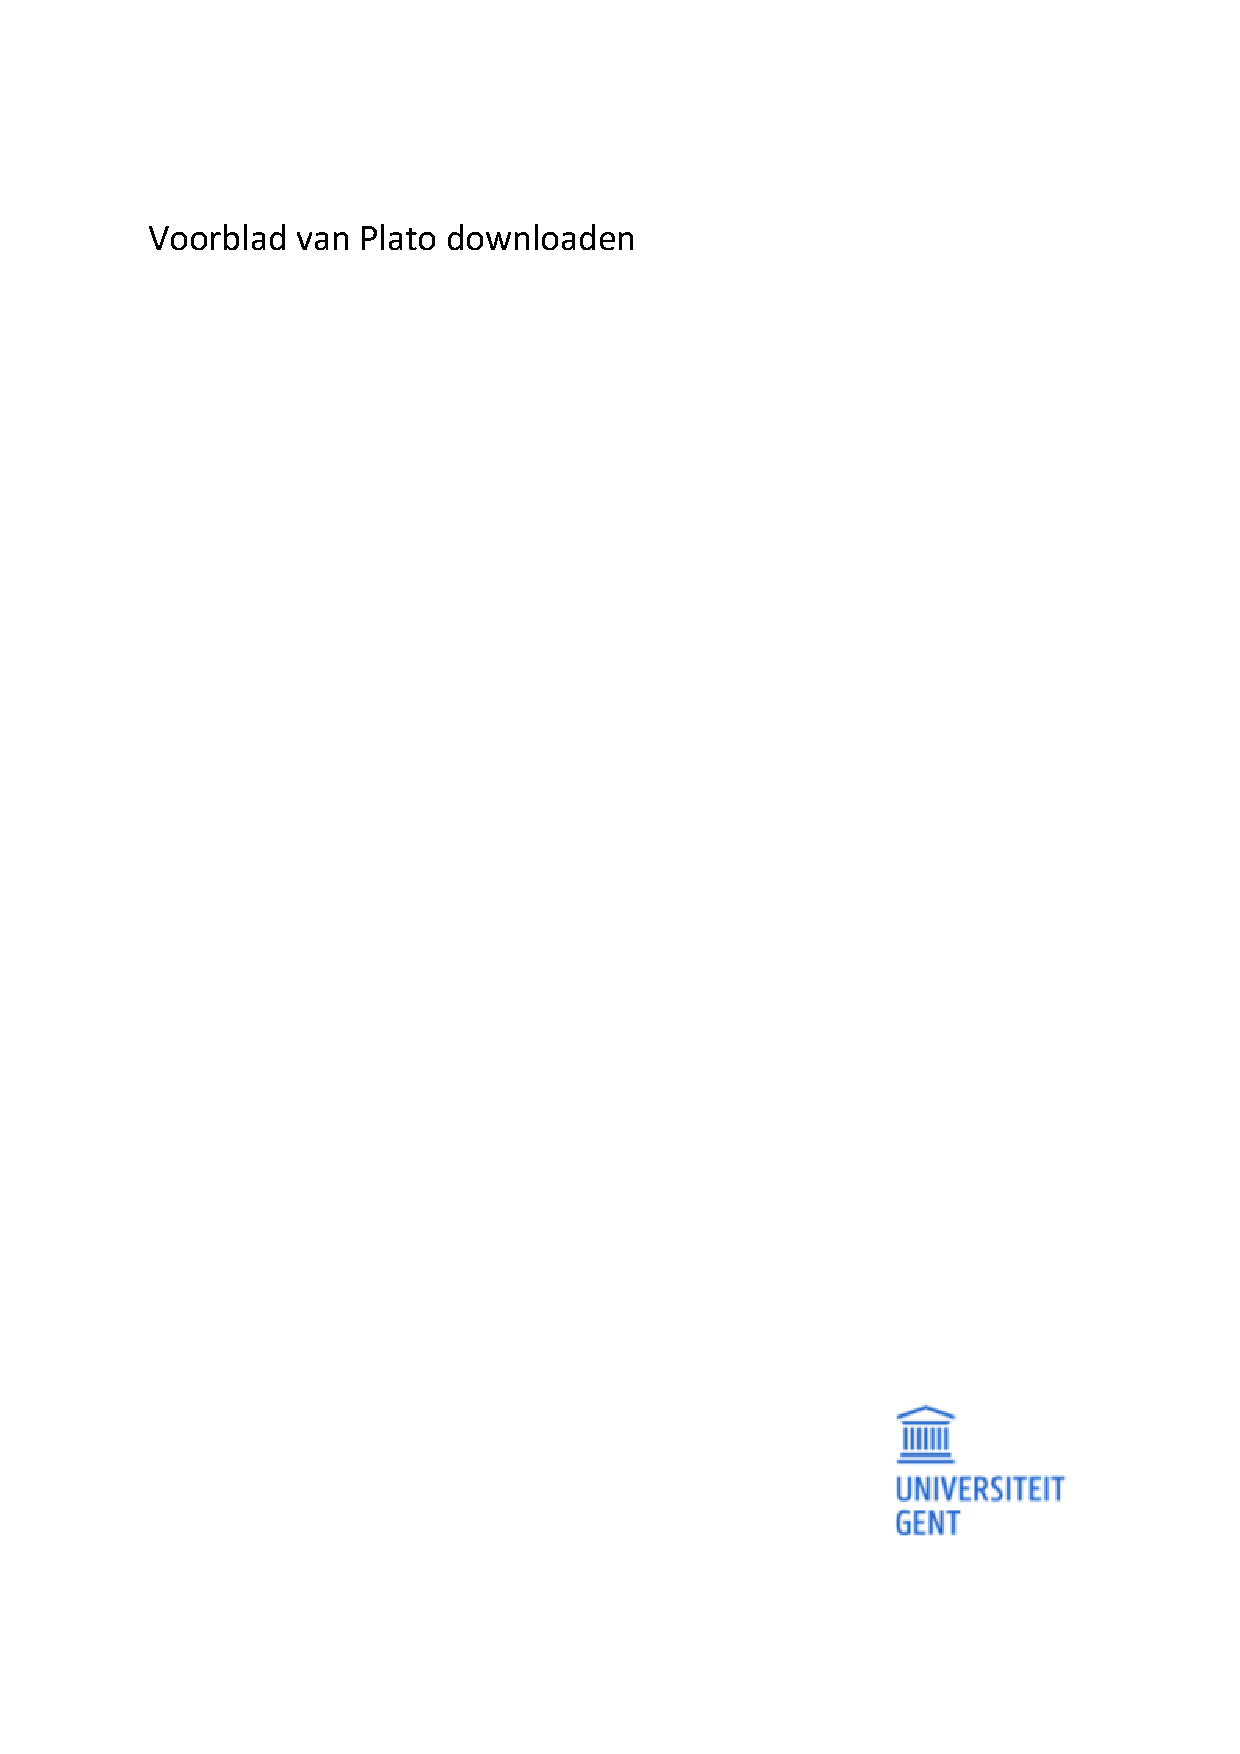
\includepdf{cover-sheet.pdf}

\chapter*{Dankwoord}

Allereerst wil ik mijn promotoren, prof. dr. Bruno Volckaert en prof. dr. ir. Filip De Turck, en begeleiders, dr. ing. Merlijn Sebrechts en dr. ing. Tom Goethals, bedanken. Zonder hen zou deze masterproef nooit tot stand gekomen kunnen zijn. In het bijzonder wil ik dr. ing. Merlijn Sebrechts bedanken voor de opvolging en het oneindige geduld om mijn zinnen met een passive voice aan te duiden. 

Daarnaast wil ik graag mijn ouders bedanken voor de steun, en het proeflezen. Zonder hen zou dit ook nooit tot stand gekomen kunnen zijn en waren er ongetwijfeld nog talloze grammaticale fouten aanwezig. 

Tot slot wil ik ook graag iedereen in de Bytecode Alliance waarmee ik in contact gekomen ben bedanken voor diens onschatbare feedback en hulp, hieruit wil ik Dan Gohman, Chris Woods en Maximilian Seidler uitlichten.

\chapter*{Permission for Usage}

The author gives permission to make this master’s thesis available for consultation and to copy parts of this master’s thesis for personal use. Every other use is subject to copyright terms, in particular with regard to the obligation to explicitly state the source when quoting results from this master’s thesis.


\chapter*{Abstract - Dutch}
\chaptermark{Abstract - Dutch}
\addcontentsline{toc}{chapter}{Abstract - Dutch}


\chapter*{Abstract - English}
\chaptermark{Abstract - English}
\addcontentsline{toc}{chapter}{Abstract - English}



% How to add the extended abstract:
%
% You should write the extended abstract as a separate overleaf project. Then compile it there, download the PDF, and upload it to this project.
%
% Use the "IEEE conference proceedings template" to create the extended abstract project. 
% https://www.overleaf.com/latex/templates/ieee-conference-template/grfzhhncsfqn
%
% Then download the final PDF, upload it to the root of this project, and point the statement below to the correct file.


% How to add the extended abstract:
%
% You should write the extended abstract as a separate overleaf project. Then compile it there, download the PDF, and upload it to this project.
%
% Use the "IEEE conference proceedings template" to create the extended abstract project. 
% https://www.overleaf.com/latex/templates/ieee-conference-template/grfzhhncsfqn
%
% Then download the final PDF, upload it to the root of this project, and point the statement below to the correct file.

\tableofcontents\newpage
\listoffigures\newpage
\listoftables\newpage
%%%%%%%%%%%%%%%%%%%%%%%%%%%%%%%%%%%%%%%%%%%%%%%%%%%%%%%%%%%%%%%
%                                                             %
% Note: To add or remove acronyms, modify `personal_data.tex` %
%                                                             %
%%%%%%%%%%%%%%%%%%%%%%%%%%%%%%%%%%%%%%%%%%%%%%%%%%%%%%%%%%%%%%%

% Print the glossary
% \printglossary[type=\acronymtype, title={Lijst van afkortingen}]
\printglossary[type=\acronymtype, title={List of Acronyms}] % English

\glsaddallunused[\acronymtype]                              % make sure all unused acronyms are in list

\setlist[description]{style=standard} % reset list settings back to default

% list all code listings
\listoflistings\newpage
\newpage

%
% Include the main chapters of the thesis below
% Note: it's best to avoid spaces in filenames as Latex might complain about them.
%
\mainmatter
\pagestyle{fancy} % Use header
% Moet zeker goed verwoord zijn
\chapter{Introduction}
\label{chap:intro}

[secties zijn tijdelijk, en puur om aan te tonen dat tekst voor "onderzoeksvragen" nog niet klaar genoeg is]
\section{WIP}
% Dit kan gezien worden als een omgekeerde driehoek

% 1. Wat is het maatschappelijke probleem?
% 	1. Voorbeeld: Updaten van auto's
% 	2. Er mag gelinkt worden met nieuwsartikels

There are countless software solutions running on critical hardware, where sudden failure could result in the loss of people's live, e.g. programs guiding surgeons during operations or cars. Furthermore, in the case of cars, there's a clear trend towards more advanced infotainment systems and to update these remotely without the need to visit an auto mechanic. When such an update fails to perform, it should be possible to rollback unbeknownst to the driver.

% TODO: Brug naar lange termijn onderhoud
% 2. Firmware, heel lang onderhouden en zo brugje naar Wasm maken
% 	1. Probleem: Wasm heeft geen manier om met hardware te praten
% 	2. En dan dit probleem uitdiepen: Wasi, I2C

In addition, with the advent of generational AI's like ChatGPT, worldwide GPU usage has exploded. Directly translating in an explosion of energy and water usage to run all and cool all this harware inside data-centres. Sadly, these GPUs have long-lasting periods of idly running, waiting for requests. It should be possible to start a GPU when running a request, but otherwise keep it off, without significant overhead in terms of latency.

% TODO: Hierop is de hele korte startup times en overhead van Wasm ook de oplossing

\section{Onderzoeksvragen}
% TODO: 3. Onderzoeksvragen en kort overzicht
% 	1. Hoe kan het secure gebeuren?
% 	2. Wat is de performance?


% \setcounter{page}{1}

\chapter{I2C fundamentals}
\label{chap:i2c}

As we will be leveraging the \gls{I2C} protocol, it is worth looking into the inner workings. 

\gls{I2C}~\cite{nxp:i2c} is a serial communication bus invented in the eighties by Philips Semiconductors. It uses only two bidirectional lines, a \gls{SDA} and a \gls{SCL}. Typically, 7-bit addressing is used, but there exists a 10-bit extension. This extension is fully backwards compatible, allowing a software-emulated 10-bit addressing implementation if the hardware only supports 7-bit addressing.

This communication bus has no minimum frequency, but can go as fast as 5 Mbit/s. Not every \gls{MCU} supports every frequency though, for example the PCF8523 Real-Time Clock only supports up to 1 MHz.

Besides a 0 or 1 data bit, there are two special START and STOP signals which act as message delimiters.

% [in principe kan er nog verteld worden over de verschillende snelheden en dergelijke, maar aangezien ik daar niet mee te maken heb gehad ben ik van mening dat dat hier out of scope is]
\section{Operations}

A node on the bus can have one of two roles\footnote{In earlier literature, the terminology master and slave were used for respectively controller and target.}:
\begin{itemize}
    \item Controller: Generates the clock, via required minimum periods for the low and high phases of the \gls{SCL}, and initiates communication with targets.
    \item Target: Receives the clock and responds when addressed by the controller.
\end{itemize}
Any number of any type can be present, and these may be changed between messages. They can also both receive and send data, when in the corresponding mode.

Initial communication is established by a controller that sends a START followed by the address of the target it wishes to communicate with, which is finally completed by a single bit indicating if it wishes to write (0) or read (1) from the target. If the target exists on the bus, it will respond with an acknowledgement. This \gls{ACK} corresponds with transmitting a single 0 bit, there is also a \gls{NACK} which is a single 1 bit.

\begin{figure}[h]
    \centering
    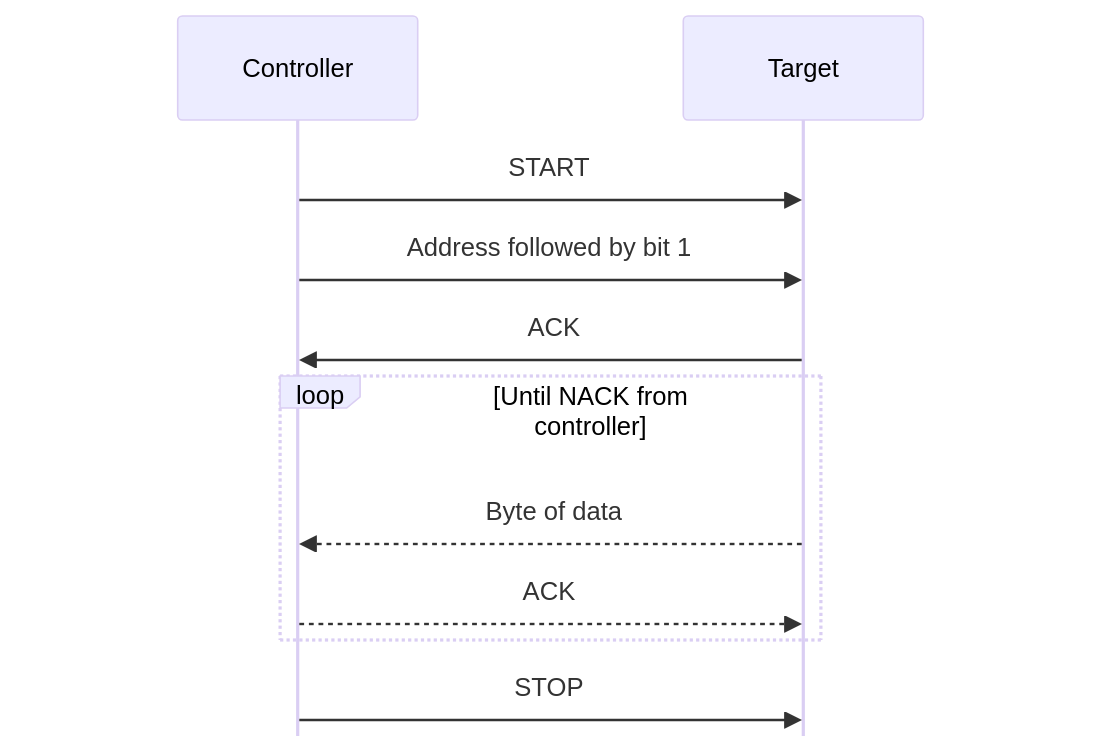
\includegraphics[width=0.5\textwidth]{figures/read_example.png}
    \caption{Example sequence of a read operation.}
    \label{fig:read_example}
\end{figure}

Further communication is performed by one party sending data, most significant bit first, and the other sending an \gls{ACK} bit.

\subsection{Bus sharing}

In the case of multiple targets linked with one controller, the controller needs to indicate which target it wants to interact with. To achieve this, each target compares the address sent by the controller with its own. If the address matches, it sends a low voltage \gls{ACK} bit back to the controller. If the address doesn't match, the target does nothing and the \gls{SDA} line remains high.

When there are multiple controllers, issues can arise, precisely when they try to send or receive data at the same time over the \gls{SDA} line. To solve this problem, each controller needs to detect if the \gls{SDA} line is low or high before transmitting a message. If the \gls{SDA} line is low, another controller is in control of the bus, and it should wait until a STOP has been received to send the message. If the \gls{SDA} line is high, then it's safe to transmit the message.

\subsection{Methods}

The protocol defines three basic types:
\begin{itemize}
    \item Write: Controller writes bytes to the target.
    \item Read: Controller reads bytes from the target until a given buffer is full.
    \item Write-read: Controller first writes bytes and then reads enough bytes to fill the buffer in a single transaction.
\end{itemize}

It is also possible to combine a list of write and read operations inside a transaction contract.
Figure \ref{fig:read_example} showcases more in detail how a read operation works.

\section{SMBus}
% [het idee is dat er hier uitgelegd gaat worden van wat SMBus is en de relatie met I2C]

The \gls{SMBus}~\cite{smbus} is a subset derived from \gls{I2C} by Intel. Its main application is to monitor critical parameters on PC motherboards and in embedded systems. On the surface they are quite similar, but there are some subtle differences worth mentioning. For one, \gls{SMBus} will time out when \gls{SCL} is held low for more than 35 milliseconds. \gls{I2C} doesn't have an established timeout value, implicating that a target or controller can hold \gls{SCL} as long as necessary to process data. \\
On account of this timeout, \gls{SMBus} has a minimum clock speed of 10 kHz. Leading to a maximum of 100 kHz. As stated earlier, \gls{I2C} can go as fast as 5 Mbit/s and no minimum frequency is specified.

Another difference is in terms of voltage levels. For \gls{I2C} the typical levels are +5 V, +3.3 V or even +1.8 V and below. In contrast, in an \gls{SMBus} system the supply ranges are restricted between +1.8 V and +5 V. In general, even with the different specifications for the input logic voltage thresholds, \gls{I2C} and \gls{SMBus} devices will be interoperable over the supply voltages permitted by the SMBus specification.

Sometimes libraries that provide methods for \gls{I2C} communication, also provide ones for \gls{SMBus}. But, thus, in the context of driving an \gls{I2C} target device, these can be safely ignored.


\chapter{Interfacing hardware}
\label{chap:hardware}
% [Deze sectie draait rond HAL, wat het is, waarom het nodig is en waarom het nuttig is om een gelijkaardige API te voorzien. Ter inspiratie kan de \verb|embedded_hal| scope en design goals genomen worden.]

Embedded devices have a high degree of diversity of possible constraints, e.g. 64-bit support, memory size and the availability of hardware units like a memory protection unit. Making it difficult for drivers to support any number of target platforms, unless these platforms are abstracted away behind a shared API. This is the purpose of a \gls{HAL}. It is important that this layer hides device-specific details and that it is generic across devices. 

For Rust, this \gls{HAL} is, aptly, named \href{https://github.com/rust-embedded/embedded-hal}{embedded-hal} and provides traits for using peripherals commonly available in microcontrollers such as \gls{GPIO}, \gls{UART}, \gls{SPI} or \gls{I2C}. There exists many crates that implement these interfaces for a certain microcontroller family or a system running some \gls{OS}. Furthermore, there are also loads of driver crates that use the \texttt{embedded-hal} interface to support all these families and systems. A curated list can be found in the \href{https://github.com/rust-embedded/awesome-embedded-rust}{Awesome Embedded Rust} repository.

Sadly, the notion of a community-wide shared interface is not universally present in all embedded communities. The C/C++ community is such an example, where there isn't one \gls{HAL} to rule them all.

\section{Different versions of \texttt{embedded-hal}}

Unfortunately, there are two major versions of \texttt{embedded-hal}, i.e. $0.2.7$ and $1.0$, which are incompatible with one another. 
As version 1.0 was only released on the ninth of January 2024, it is still fairly novel. Thus, crates have a wildly varying degree of compliance with this version. 

Broadly speaking, there are four major changes \cite{hal:1}. Firstly, traits have been simplified and others have been merged to remove interopability gotchas. 
Secondly, async versions of the blocking traits are now available in the \texttt{embedded-hal-async} crate. Thirdly, there is now support for \gls{SPI} bus sharing. Lastly, there is improved error handling.

There is \href{https://github.com/ryankurte/embedded-hal-compat}{a crate} that tries to provide a compatibility layer between these two versions, but the latest supported version is merely a release candidate of $1.0$. Thus, the crate is not really practically useful.

\section{Peripheral Access Crates}

\gls{SVD} files are \texttt{XML} files typically provided by silicon vendors which descibe the memory map of a device. Via \href{https://crates.io/crates/svd2rust}{the \texttt{svd2rust} crate} it is possible to generate a mostly-safe Rust wrapper. Further discussion is out of scope as this is a very thin wrapper, and usually depended upon by \gls{HAL} authors.

\section{Running the solution}
\label{sec:running}

When the target platform is an \gls{OS}, it is typically fairly easy to build and execute a software solution, plainly by doing this on the target device itself, or by cross-compilation from a morepotent device. This is not the case for an \gls{MCU}, here, only cross-compilation is possible. Due to the constrained nature of memory on an \gls{MCU}, the memory-layout also needs to be specified.

In the case of a Raspberry Pi Pico, compilation results in an \texttt{UF2} and an \texttt{ELF} file. The former is a file format developed by Microsoft for flashing microcontrollers over mass storage connections. The latter is used by the debugger.

To pogram the flash on the Pico, the \texttt{BOOTSEL} button needs to be held. Forcing it into USB Mass Storage Mode. Then, you can move a \texttt{UF2} file onto it. Whereupon the \texttt{RP2040} processor of the Pico will reboot, unmount itself, and run the flashed code. Other boards could require pulling down the flash \texttt{CS} pin, which is how the \texttt{BOOTSEL} button works on the pico, using an exposed \gls{SWD} interface, also an option for the Pico, or have a reset button that needs to be double-pressed.

\gls{SWD} is a standard interface on Cortex-M based microcontrollers, which the host machine can use to reset the board, load code into flash, and set the code running. Without the need to manuallyl reset the board or hold the \texttt{BOOTSEL} button. The easiest way to connect with this interface on a Pico is to make use of a debug probe via \href{https://probe.rs/}{probe-rs}. This also unlocks the ability to print to \texttt{STDOUT} or even utilize the \href{https://microsoft.github.io/debug-adapter-protocol/overview}{Debug Adapter Protocol}.


\chapter{WebAssembly}
\label{chap:wasm}
% [Algemene uitleg van wat WebAssembly is en waarom we het buiten het web willen kunnen gebruiken. Hiervoor wordt er dan verwezen naar de lagere memory footprint ten opzichte van docker. Alsook moet er verteld worden wat de previews zijn en de timeline van wanneer ze gereleased zijn. Spinup time is ook een zeer belangrijke om te vermelden.]

\gls{Wasm} is a binary instruction format for a stack-based \gls{VM}. It is designed as a portable compilation target for programming languages. Binaries have a \texttt{.wasm} file extension, there's also a textual representation which has a \texttt{.wat} extension. This enables deployment on the web for client and server applications. Examples of web applications using this technology are \href{https://photoshop.adobe.com/}{Adobe Photoshop} or \href{https://earth.google.com/web}{Google Earth}.

Although the name implies it, \gls{Wasm} is not merely limited to the web. There are runtimes that enable execution on a myriad of platforms, ranging from Linux devices to smartphones or even microcontrollers. All possible through the usage of a system interface, called \gls{WASI}.

\section{WebAssembly System Interface}
\label{sec:wasi}

\gls{WASI}~\cite{wasi} is a modular collection of \gls{API}'s defined with the \gls{WIT} IDL, see section~\ref{sec:wit}, that provide a secure and portable way to access several operating-system-like features such as filesystems, networking, clocks and random numbers. This collection is developed under the governance of the \gls{WASI} Subgroup, a subgroup of the WebAssembly Community Group.

In this subgroup, the following design principles are core:

\begin{itemize}
    \item Capability-based security: All access to external resources is provided by capabilities, see chapter~\ref{chap:component_model}.
    \item Interposition: A Webassembly instance can implement a given WASI interface, and the consumer WebAssembly instance can then use this implementation transparently.
    \item Compatibility: If possible, keep the \gls{API} free of Compatibility concerns, and provide compatibility through libraries.
    \item Portability: The exact meaning of this is specific to each \gls{API}, but in globo it means that no engine should need to implement every \gls{API} in \gls{WASI}.
    \item Modularity: The component model's worlds mechanism is used, in order to allow specific sets of APIs to be described which meet the needs of different environments. See chapter~\ref{chap:component_model}.
\end{itemize}


% [Hier vergelijking met docker doen.]

\subsection{Versions}
\label{sec:versions}

Originally \gls{WASI} launched under the name: \texttt{WebAssembly System Interface, snapshot 1}, nowadays called \texttt{0.1} or \texttt{Preview 1}. On the twenty-fifth of January 2024, \texttt{Preview 2} was launched. Following up will be a \texttt{Preview 3}, and then the \texttt{1.0} release.

The flagship feature that \texttt{0.2} brought to the table is the component model, see chapter~\ref{chap:component_model}. Furthermore, two \gls{WIT} worls, see section~\ref{sec:wit}, are now included:

\begin{itemize}
    \item \texttt{wasi-cli}: A command-line interface, roughly corresponding to \texttt{POSIX}.
    \item \texttt{wasi-http}: An \texttt{HTTP} proxy.
\end{itemize}

The major banner of the upcoming \texttt{0.3} is asynchronous support. The exact details of what this asynchrony entails is yet to be determined.

\section{Community}
\label{sec:community}

As mentioned in section~\ref{sec:wasi}, standardization is performed under the supervision of the \gls{WASI} Subgroup. As a part of W3C's WebAssembly Community Group, it is the key player in the standardization process. With respect to the implementations, this is the \href{https://bytecodealliance.org/}{Bytecode Alliance}, a nonprofit organization of companies. Not every company wishes to part of these bodies, e.g. \href{https://wasmer.io/}{Wasmer}, [zijn er nog goede voorbeelden?].

\section{Runtimes}
\label{sec:runtimes}
% [Wasmtime uitvoerig bespreken, maar ook de meest belangrijke andere runtimes. Het is niet de bedoeling om echt in depth te gaan vergelijken en te benchmarken, maar om gewoon wat te schetsen wat er allemaal is. Daarnaast ook vertellen in welke mate, en hoe, je een preview2 component op een runtime kan laten draaien dat geen support heeft voor het component model. Misschien ook kort iets rond changes die in Wasmtime kunnen gebeuren om meer embedded devices te supporten.]

A runtime system is an infrastructure that participates in the creation and running of \gls{Wasm} binaries. Typically, the components of this are the execution environment, or application \gls{VM}, to provide a place for the program to run, the compiler front-end and/or the compiler back-end for the necessary analysis, transformations and optimization.

The Bytecode Alliance fosters two runtimes, \href{https://github.com/bytecodealliance/wasmtime}{Wasmtime} and \href{https://github.com/bytecodealliance/wasm-micro-runtime}{WAMR}. The former can be seen as a more general-purpose runtime, focussing on server-side and non-web embeddings with components. Making it the de-facto runtime. While \gls{WAMR} specifically is designed to be as lightweight as possible, targeting embedded devices and the edge. This translates itself into the provided features and the supported guest languages. For example, Wasmtime has full component model support, while \gls{WAMR} has it planned for end of 2024. With regards to the supported languages, \gls{WAMR} only supports C/C++. A toolkit for Rust has been published in March 2024. On the other hand, Wasmtime has first-class support for eight languages, and community support for a further two. Furthermore, there's active effort in making this runtime lighter to run. One such effort is the inclusion of a Rust \texttt{no\_std} option.

Besides these two there are numerous ones provided by other parties, in varying degrees of completeness, targeting other use-cases. There's for example \href{https://github.com/bytecodealliance/jco}{jco}, specialized for JavaScript, \href{https://github.com/bytecodealliance/componentize-py}{componentize.py}, for Python, or \href{https://github.com/dylibso/chicory}{Chicory}, which runs on the Java \gls{VM}. 

\chapter{The Component Model}
\label{chap:component_model}

% [Wat is het component model en waarom willen we het. Ook vertellen dat je het kan zien als een guest/host-architectuur, maar dat het perfect mogelijk is om meerdere componenten samen te weven.]

The WebAssembly Component Model is an architecture for building interoperable \gls{Wasm} liraries, applications and environments. These components can be seen as containers for modules, or other components, which express their interfaces and dependencies via \gls{WIT} and the canonical \gls{ABI}. 
An \gls{ABI} can be seen as an agreement on how to pass around data in a binary format, specifically concerned with the data layout at the bits-and-bytes level. The Canonical \gls{ABI} defined by the component model, specifies how the \gls{WIT} type definitions are translated to bits and bytes. Internally, a C and a Rust component might represent strings in a quite different way, but the canonical \gls{ABI} provides a format for them to pass strings across the boundary between them.

It is important to note, though, that the Component Model is not \gls{WASI} (\texttt{Preview 2}), nor a part of it. By way of comparison to traditional \gls{OS}, the Component Model fills the role of an \gls{OS}'s process model, defining how processes start up and communicate with each other, while \gls{WASI} fills the role of an \gls{OS}'s many I/O interfaces.

It is easiest to think of the Component Model as a guest-host architecture, but it is certainly possible to compose multiple components together. For this, \href{https://github.com/bytecodealliance/cargo-component}{cargo-component} can be used in Rust, or the language-agnostic \href{https://github.com/bytecodealliance/wasm-tools}{wasm-tools}.

\section{WIT}
\label{sec:wit}
% [Schetsen wat WIT is en kort hoe de syntax in elkaar zit. Misschien dat het ook handig kan zijn om uit te leggen hoe dependencies in WIT gemanaged worden.]

\gls{WIT} is an \gls{IDL}. This means that it is a format that defines how the interface of a component should look like. To this end, it uses the following set of concepts: types, functions, interfaces, worlds and packages. From these, worlds are the most key.

A world describes the capabilities and needs of a component - it says which interfaces are available for outside code to call, the \texttt{export}s, and which interfaces it depends on, the \texttt{import}s. Thus, only the surface of a component is defined, not the internal behaviour. The internal behaviour is determined when the world is targeted by a component an application or library developer creates. For a component to run, its imports must be fulfilled, by a host or by other components. \\
On the other hand, a world defines an environment in which a component can be instantiated and its functionality can be invoked.

There are also some small intricacies worth pointing out. For types, two things stand out. First, both the \texttt{char} and \texttt{string} types are Unicode. Second, there's the user-defined \texttt{resource} type. This type can be seen as an object that implements an interface, and therefore behaviour is only exposed through methods. \\
Furthermore, functions can only be declared as part of an interface, or as an import or exprot in a world. Finally, a package is not a world, but can be seen as more like a namespace. It's a way of grouping related interfaces and worlds together for ease of discovery and reference.


To make managing dependencies inside your \gls{WIT} definition easier, the \href{https://github.com/bytecodealliance/wit-deps}{wit-deps} project can be used. It makes it possible to lock your dependencies to a certain version and to check if they're the most recent one.

\subsection{\texttt{witx}}

In older tooling, it is possible to come across \texttt{witx} instead of \gls{WIT}. This was the \gls{IDL} used during \texttt{Preview 1}. It was derived from \texttt{wat}, see chapter~\ref{chap:wasm}, and had a low-level C-like type system that emphasized raw pointers, and callees were expected to have access to the entir lineair memory of the caller.
 
\section{Guest}
\label{sec:guest}
% [Op welke manieren kan je allemaal code schrijven dat dan naar een preview 2 component gecompileerd kan worden. Verschillende tooling over programmeertalen heen de specifieke voor Rust. Alsook hoe we van preview1 component naar preview2 kunnen gaan.]

In Rust, \texttt{cargo-component} can be used to compile code to a preview 2 component. In essence, compiling to \texttt{Preview 2} means compiling to \texttt{wasm32-wasi} and then converting it to a component via an adapater and the \texttt{wasm-tools component new} subcommand. This component then adheres to the \gls{WIT} interface specified in the configuration file. The adaption is needed because there's no first-class support for \texttt{Preview 2} yet. Mainstream support for this is planned for early 2025~\cite{rust:p2}.

Under the hood, \texttt{cargo-component} relies upon \href{https://github.com/bytecodealliance/wit-bindgen}{wit-bindgen} for binding with the interface. Besides Rust, \texttt{wit-bindgen} also supports the following languages: C, Java, Go and C\#. For JavaScript, \href{https://github.com/bytecodealliance/ComponentizeJS}{ComponentizeJS} can be used.

\subsection{Adapter modules}

The Wasmtime runtime publishes adapter modules with each release, they provide the bridge between the \texttt{Preview 1} \gls{ABI} and the \texttt{Preview 2} \gls{ABI}. The following three modules are provided:

\begin{itemize}
    \item Command: For command-line applications
    \item Reactor: Applications that don't have a \texttt{main} function
    \item Proxy: For applications fed into \texttt{wasmtime serve}
\end{itemize}

The \texttt{wasmtime serve} subcommand runs a component inside the \texttt{wasi:http/proxy} world, supporting the sending and receiving of HTTP requests.

\section{Host}
\label{sec:host}
% [Uitlegen dat je runtimes hebt en dat je rechtstreeks daarop kan draaien of dat er ook visence, compiling to preview 2 means compiling to \gls{Wasm} and then converting it to a component via an adapater.

The job of the host is to load a component and execute it through the usage of a \gls{Wasm} runtime. See section~\ref{sec:runtimes} for a shortlist of the available ones. To guarantee a correct execution, it is important to make sure that any missing interface imports are filled in here, see the earlier section~\ref{sec:wit}. When using \texttt{wit-bindgen}, this is done via the \texttt{with} option inside the \href{https://docs.rs/wasmtime/latest/wasmtime/component/macro.bindgen.html}{the \texttt{bindgen} macro}.

It is also possible to execute a component via the \texttt{wasmtime run} subcommand. This will compile the module to native code, instantiate it and optionally execute an export.


\section{Problems}
% [hier iets vertellen over dat het gebruik maken van het component model wel wat nadelen inhoudt, zoals extra geheugen dat nodig is enzo, waardoor het niet altijd gewenst is voor dit te gebruiken. Of toch zeker momenteel op hele zwakke MCU's]

[Hier kan er misschien iets verteld worden over de argumenten om component model niet te gebruiken? Is dit wel nuttig en willen we dat wel?]

\chapter{Architecture and standard}
\label{chap:architecture}
% [Vertellen over de proposal, hoe championship werkt, wat de huidige status is en wat er moet gedaan worden om het te advancen. Daarnaast ook de laatste status rond SIG Embedded vertellen en de missie ervan.]

% 1. Primer om te vertellen wat nodig is om dan de rest te snappen
As stated previously in section~\ref{sec:wasi}, \gls{WASI} is a collection of \gls{API}'s. In order for \gls{I2C} support inside \gls{WASI}, an \gls{API} should thus be defined and standardized. The \gls{API} is publicly available inside the \href{https://github.com/WebAssembly/wasi-i2c}{wasi-i2c} repository.

Software developed without any reviews, nor feedback, is software that is doomed to fail at some point. The same principle applies to the standardization of a proposal. For feedback, the input from the \gls{Wasm} community, see section~\ref{sec:community}, is invaluable. Besides this community, there's also a subcommunity of people interested in the combination of \gls{Wasm} and embedded devices. To ratify this subcommunity, a request for a \gls{SIG} Embedded has been opened with the Bytecode Alliance.

\section{The proposal process}

Stated in section~\ref{sec:wasi}, \gls{WASI} is under the goverance of the \gls{WASI} Subgroup. This subgroup is further split up into the Community Group and the Working Group. The purpose of the Community Group is to attempt to address all concerns, but no 100\% consensus is needed. The Working Group, on the other hand, is there to finalize and ratify mostly complete specifications plus test suites from the Community Group.

% This means that they are responsible for any proposed changes to this collection of interfaces to be thoroughly vetted by the community.

The process is split up into five stages of standardization:

\begin{description}
    \item[Phase 0.] Pre-Proposal: The Community Group decides whether the pre-proposal is in scope for \gls{WASI}.
    \item[Phase 1.] Proposement of the feature: An overview document must be produced that specifies the feature with reasonably precise and complete language.
    \item[Phase 2.] Specification text is available: A test suite should be added, and it should pass on the prototype or some other implementation.
    \item[Phase 3.] The specification gets implemented by engines.
    \item[Phase 4.] The feature is being standardized: Ownership gets transferred from the Community Group to the Working Group, and two or more Web \gls{VM}'s have implemented the feature.
    \item[Phase 5.] The feature is standardized: Editors perform final editorial tweaks and merge the feature into the main branch of the primary specification repository.

\end{description}

To go from the one stage to the following, a vote in the subgroup needs to be passed. Except to enter phase 0, here the proposal is still merely an idea.

It is the convention that a proposal has the \texttt{wasi-} prefix. This is the reason the \gls{I2C} proposal is called \texttt{wasi-i2c}.

\subsection{Current \texttt{wasi:i2c} phase}

Currently, the \gls{I2C} proposal is in the first phase, with ongoing effort to fullfill the criteria to pass the vote to the second phase. Specifically, a broad enough of a consensus needs to be reached on the capability criteria. This effort is led under the guidance of certain champions. For \texttt{wasi:i2c} these are Friedrich Vandenberghe, Merlijn Sebrechts and Maximilian Seidler. Both Friedrich and Merlijn are from UGent, Maximilian is from Siemens. This mix of academians and people from the industry ensures ongoing standardization effort and actual usage of the feature.

\section{Alternatives to Wasm}

% 2. Bredere exploratie voor alternatieve oplossingen
% 	1. Hoe I2C aangesproken wordt vanuit nodejs (antwoord: ze geven linux handle) en via linux
% 	2. WebUSB: Dit is via js dus barf
% 	3. Hier kan er hard gegaan worden op linken met academische artikels


% Vanaf hier mag er geen nieuwe kennis meer geïntroduceerd worden!
\chapter{Implementations}
\label{chap:implementation}
% [De hele hardware setup uitleggen, dus de verschillende Pi's en de apparaten waar er mee gepraat wordt.]
As stated in chapter~\ref{chap:architecture}, it is necessary to provide implementations to ascertain the soundness of the \gls{WIT} interfaces. Ideally, these are as diverse as possible. Both in terms of operations on the \gls{I2C} connection, and the target architectures.

Three implementations are provided: one that performs an \gls{I2C} read and two that write to an \gls{I2C} connection, developed for three devices targeting two architectures. 
On the one hand, we have a Raspberry Pi 3 and 4 targeting ARM64 Linux, and on the other hand we have a Raspberry Pi Pico \gls{MCU} targeting RP2040 processor.

% TODO: DHT22 en ESP8266 opzoeken
On the Pi 3, a \gls{HAT} is mounted that contains a HTS221 sensor, from which the current temperature and humidity is read. The Pi 4 is either connected with a HD44780 LCD character display or a 4-digit 7-segment display. 
Although the Pi 3 could also be linked up with these displays, it's more of a hassle thanks to the \gls{HAT}. The pico is solely linked with the 4-digit display. Because of the \gls{MCU} constraints, controlling the HD44780 is out of scope.

\begin{figure}[h]
    \centering
    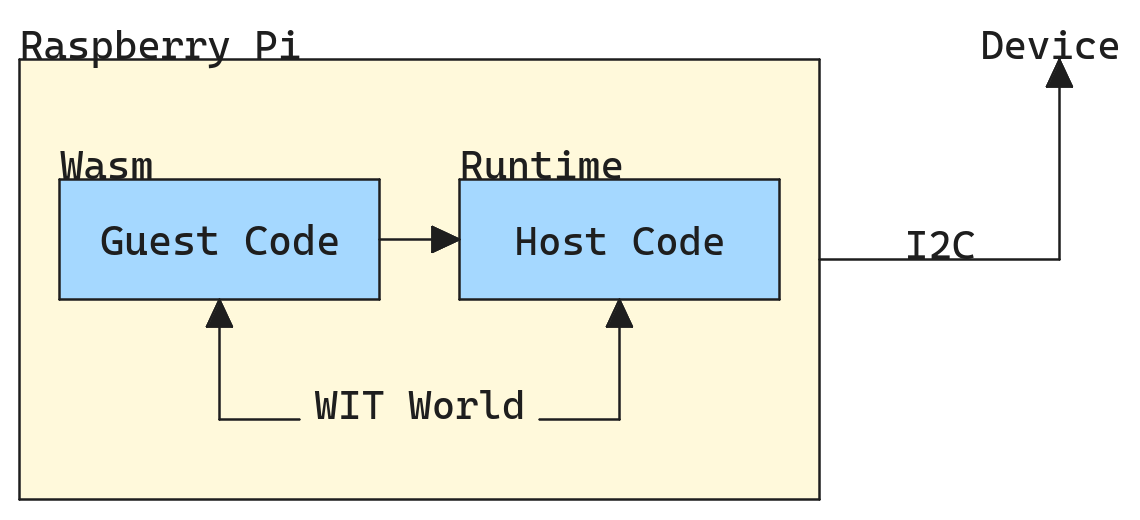
\includegraphics[width=0.5\textwidth]{figures/schema.png}
    \caption{Schematic overview of an implementation.}
    \label{fig:schematic}
\end{figure}

Conceptually, each implementation comes down to the schematic defined in figure~\ref{fig:schematic}. Only the guest code differs for each device. See chapter~\ref{chap:wasm} for an in-depth explanation.

% TODO: Hier foto's zetten van de verschillende setups

\section{Embedded driver development in Rust}
% [Native driver development, hoe gaat het te werk en de grote verschillen voor native development voor een gewone Pi en een microcontroller zoals de Pi Pico.]
Besides the implementation itself, two things are of significance to design a device driver in Rust. Namely, following the Embedded \gls{HAL} \gls{API}, see chapter~\ref{chap:hardware}, and supporting the desired target architecture.

Fortunately, Rust provides support for a great deal of platforms. Thus, building for ARM64 is as simple as providing the \texttt{--target aarch64-unknown-linux-gnu} flag. However, the RP2040 architecture needs special attention. For this, besides setting the \texttt{--target} flag with \texttt{thumbv6m-none-eabi}, we also need to provide a file called \texttt{memory.x}. 
This file is a linker script which specifies the memory layout of the target device, see section~\ref{sec:running}. Furthermore, the \gls{MCU} has only support for a \texttt{no\_std}.

\section{Embedded driver development in WebAssembly}
% [Om van native naar Wasm te gaan, wat moet er veranderen.]embedded-hal 0.2 vs 1.0 vermelden
Besides the considerations from the previous section, we now also need to keep the used runtime target platform support in mind. See section~\ref{sec:runtimes} for an overview. Furthermore, in this section, the different features of each runtime are also highlighted. These led to a vastly different implementation for both the host and the guest code.

\subsection{Wasmtime}

The guest is made into a component via the procedure specified in section~\ref{sec:guest}. The configured \gls{WIT} interface is the one specified in codefragment~\ref{code:wit}. 
Herein \texttt{wasi:i2c} is the proposal, as explained in chapter~\ref{chap:architecture}. Both displays are represented by the \texttt{screen} world, which needs both \texttt{i2c} and \texttt{delay} from the proposal. The HTS221 is mapped with the \texttt{sensor} world, that only needs \texttt{i2c}. Therefore, the former just includes the imports from \texttt{wasi:i2c}, while the latter only imports \texttt{i2c}.

The generated bindings have no way of knowing that they actually should follow the \texttt{embedded-hal} traits, for this the \href{https://github.com/Zelzahn/wasi-embedded-hal}{wasi-embedded-hal} crate is used.

On the side of the host, binding is done as described in section~\ref{sec:host}. Here, \texttt{wasi:i2c} is seen as a missing import, thus the \texttt{with} option is used with a data structure that implements the necessary traits.

\begin{listing}[h]
\begin{minted}[samepage]{rust}
package sketch:implementation;

interface hts {
    use wasi:i2c/i2c@0.2.0-draft.{i2c, error-code};

    get-temperature: func(connection: i2c) -> result<string, error-code>;
    get-humidity: func(connection: i2c) -> result<string, error-code>;
}

interface lcd {
    use wasi:i2c/i2c@0.2.0-draft.{i2c};
    use wasi:i2c/delay@0.2.0-draft.{delay};

    write: func(connection: i2c, delay: delay, message: string);
}

world sensor {
    import wasi:i2c/i2c@0.2.0-draft;

    export hts;
}

world screen {
    include wasi:i2c/imports@0.2.0-draft;

    export lcd;
}
\end{minted}
\caption{The \gls{WIT} interface to which guest and host bind.}
\label{code:wit}
\end{listing}

\subsection{WAMR}
% [vertellen dat ik in WAMR constrained was tot het doorgeven van simpele datatypes en dan maar met die globale connectie gewerkt heb]
As explained in section~\ref{sec:runtimes}, \gls{WAMR} is a lightweight runtime that, currently, has no support for preview 2. To sustain a pure Rust codebase, \href{https://github.com/bytecodealliance/wamr-rust-sdk}{WAMR Rust SDK} is used. This SDK provides Rust language bindings and support for passing integers and floats between the host and the guest. Note that strings can be passed via a conversion to a vector of the string code points.

As we can no longer use \gls{WIT}, nor pass a connection to the guest, we are enforced to greatly differ from the Wasmtime implementation. Therefore, we will focus us on the simpler 4-digit 7-segment display with the following conceptuel differences for \gls{WAMR}: The \gls{I2C} connection is kept global inside the host and there are now 4 arguments for the \texttt{write} function, one for each digit.


\chapter{Evaluation}
\label{chap:evaluation}

% [Benchmarks tonen en bespreken van het lezen van de temperatuur native vs in Wasm. Het is niet de bedoeling om de runtimes te benchmarken.]

% Kunnen het zien als een tweeluik:
% 1. Functionele evaluatie: Werkt het?
% 2. Niet-functionele evaluatie: Performantie

% Dit kan op twee manieren gestructureerd worden:
% - Per implementatie zeggen of het werkt en performant is
% - Eerst werkt het, alle setups overlopen en dan overzichtsgrafiekje geven
% 	- Deze manier heeft Merlijns voorkeur omdat je zo mooi meer meta kunt gaan

% Moet zeker goed verwoord zijn
\chapter*{Conclusie}
\chaptermark{Conclusie}
\addcontentsline{toc}{chapter}{Conclusie}  

[Terugblikken naar de introductie en wat ik allemaal bijgeleerd heb.]

Vertellen over SPI.
[Het nog verder advancen van de proposal enbespreken van dingen waar ik niet klaar mee geraakt ben.]

\renewcommand\bibname{References}
\bibliography{references}


\pagestyle{numberless} 
\pagestyle{empty}
\begin{appendices}
\section*{Bijlage A}
\addcontentsline{toc}{section}{Bijlage A}  

Toelichting bijlage.



\newpage
\section*{Bijlage B}
\addcontentsline{toc}{section}{Bijlage B}  

Toelichting bijlage.

\end{appendices}


\end{document}
